\section{Benotung}
\label{benotung}
Aktivieren Sie die Rubrik Benotung (s. Abb. \ref{benotung_uebungen} (1))

\subsection{�bersicht und Benotung der �bungen}
\label{ben}

\begin{figure}[ht]
\begin{center}
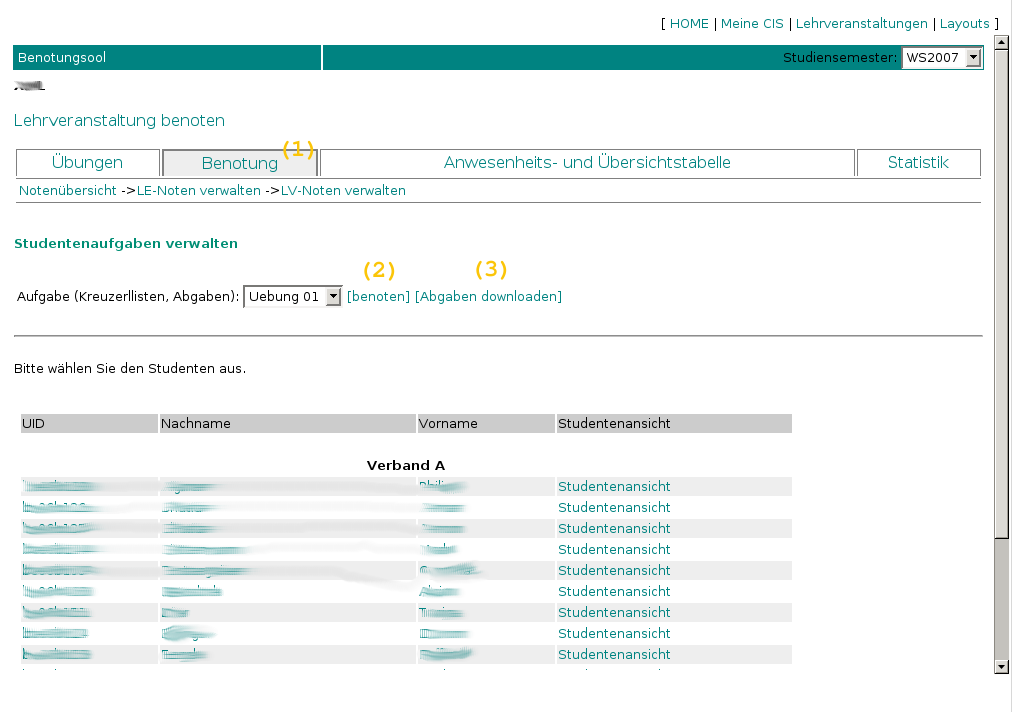
\includegraphics[width=1.0\textwidth]{benotungstool_benotung.png}
\end{center}
\caption{Benotung �bungen}\label{benotung_uebungen}
\end{figure}

W�hlen Sie eine �bung, Abgabe oder Kreuzerlliste im Dropdown-Men� aus und
klicken Sie 'benoten'(s. Abb \ref{benotung_uebungen} (2)).
Es �ffnet sich eine neue Seite mit der Liste aller
StudentInnen und einem Notenfeld oder Checkboxen f�r die Beispiele einer
Kreuzerlliste, sowie der Abgabedatei der StudentIn (s. Abb.
\ref{notenliste}).
Nehmen Sie Ihre Eintr�ge vor und speichern Sie die Seite mit
dem Knopf rechts unten ab. Schlie�en Sie die Seite.

\begin{figure}[ht]
\begin{center}
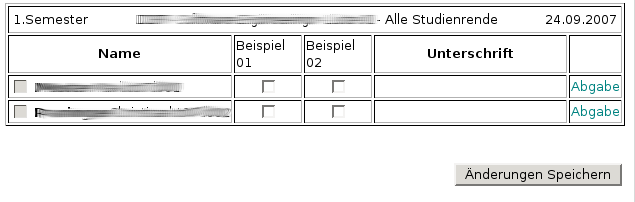
\includegraphics[width=0.7\textwidth]{benotungstool_notenliste.png}
\end{center}
\caption{Notenliste}\label{notenliste}
\end{figure}


Wenn zu einer Abgabe Studentendateien vorliegen, so wird neben dem Link
'benoten' ein weiterer Link zum Download einer ZIP-Datei mit allen Studentendateien 
dieser Abgabe aktiv (3).

Klicken Sie auf den Namen einer StudentIn, so k�nnen Sie f�r diese im Detail
Noten, Kreuzerl, Mitarbeitspunkte und Anmerkungen vergeben.\footnote{Im
Wesentlichen ist hier die Struktur des alten 'Kreuzerl-Tools erhalten geblieben'}

\subsection{Studentenansicht}
\label{studentenansicht}
F�r die Studenten in Ihrer Gruppe k�nnen Sie durch klicken auf den Link
'Studentenansicht' (rechts neben den Namen in der Liste) in einem neuen
Fenster die Ansicht des jeweiligen Studenten anzeigen lassen. In
diesem Fesnter nehmen Sie die Idetit�t der StudentIn an, k�nnen dort alle
Funktionen so bedienen wie es auch die StudentIn kann. 

Diese Funktion ist allerdings nur f�r Sie zu �bersichts-/Demonstrationszwecken
gedacht. Verwenden Sie zum �ndern der Daten (Kreuzerl hinzuf�gen/l�schen) immer
das Lektoren-Admin-Interface wie unter Punkt \ref{ben} beschrieben!

\subsection{LE-Noten verwalten}
\begin{figure}[ht]
\begin{center}
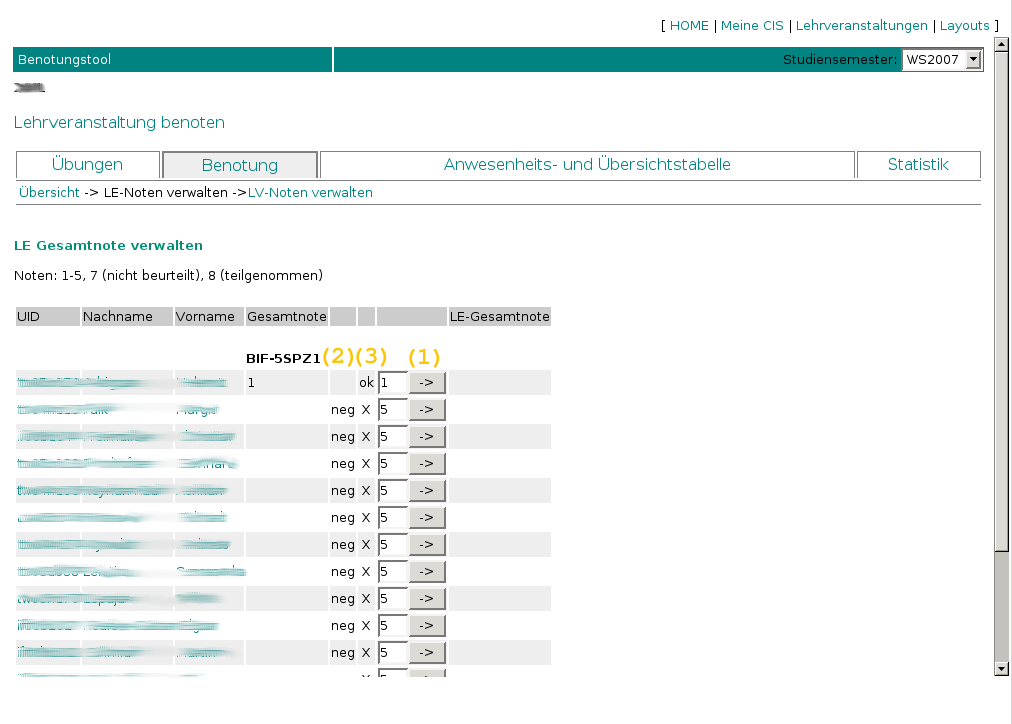
\includegraphics[width=1.0\textwidth]{benotungstool_benotung_le.png}
\end{center}
\caption{Benotung Lehreinheit}\label{benotung_le}
\end{figure}

Aus den Noten der einzelnen �bungen, Abgaben und Kreuzerllisten wird �ber die
von Ihnen definierte Gewichtung bzw. im Falle der Kreuzerllisten den
Notenschl�ssel eine Gesamtnote f�r die Lehreinheit errechnet.
Diese wird Ihnen gerundet zur �bernahme als LE-Gesamtnote vorgeschlagen.
�berpr�fen/korrigieren Sie diese und �bernehmen Sie sie mittels '-$>$' - Knopf.
(s. Abb. \ref{benotung_le} (1))

Weitere Felder:
'neg' (2) in der Spalte neben der errechneten Note bedeutet, dass zumindest als zwingend positiv
definierte Note negativ ist; 'ok'/'x' (3) zeigt an, ob alle Teilnoten verf�gbar sind.

%\section{Gesamtnote}
\label{gesamtnote}
W�hlen Sie unter \url{https://cis.technikum-wien.at} -$>$ Mein Cis -$>$ Meine LV eine Lehrveranstaltung aus. Auf der �bersichtsseite klicken Sie das Symbol 'Gesamtnote' um zur Benotungsseite zu gelangen.

\subsection{Eintragen der Note}
\subsubsection{Manuelle Eintragung der Gesamtnote}
\label{ben}

\begin{enumerate}
\item Tragen Sie die Noten ein (1) und �bernehmen Sie diese mit dem '-$>$' - Knopf
\item Nachdem Sie alle Noten eingetragen haben, k�nnen Sie diese Freigeben siehe Kap. \ref{freigabe} auf S. \pageref{freigabe}\\
\end{enumerate}

\begin{figure}[ht]
\begin{center}
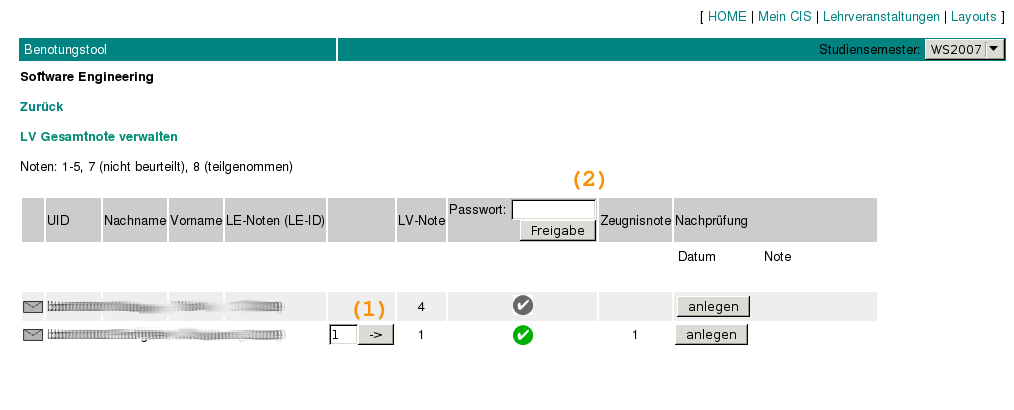
\includegraphics[width=1.0\textwidth]{benotungstool_benotung_lv.png}
\end{center}
\caption{Benotung Lehrveranstaltung}\label{benotung_lv}
\end{figure}

\subsubsection{Noten aus �bungstool (Kreuzerltool) �bernehmen}
\label{ben}

Wenn eine �bung im �bungstool (Kreuzerltool) angelegt und benotet wurde, scheint die Note in der Gesamtbeurteilung auf.
Wenn mehrere Lehreinheiten zu dieser Lehrveranstaltung vorhanden sind, wird das mittel aller Noten als Gesamtnote vorgeschlagen.

Die Notenfelder sind bereits vorausgef�llt. �bernehmen Sie diese mit dem '-$>$' - Knopf.

\subsubsection{Noten aus Moodle �bernehmen}
\label{ben}

Wenn ein Moodle-Kurs angelegt und benotet wurde, scheint die Note automatisch in der Gesamtbeurteilung auf.
Wenn mehrere Kurse zu dieser Lehrveranstaltung vorhanden sind, wird das Mittel aller Noten als Gesamtnote vorgeschlagen.
Die Notenfelder sind bereits vorausgef�llt. �bernehmen Sie diese mit dem '-$>$' - Knopf.

\subsubsection{Notenimport aus Excel}
\label{ben}

Es besteht die M�glichkeit, Noten aus einem Excel-File zu importieren. Folgende Schritte sind dazu n�tig:

\begin{enumerate}
\item Laden Sie sich die Excel-Notenliste unter CIS -$>$ Lehrveranstaltungen -$>$ Anwesenheits- und Notenlisten -$>$ Notenliste herunter
\item Tragen Sie im Excel-File die Noten ein
\item Markieren Sie im Excel die beiden Spalten Matrikelnummer und Note f�r jene Studenten f�r die Sie die Noten importieren m�chten. (ohne �berschrift)
\begin{figure}[ht]
\begin{center}
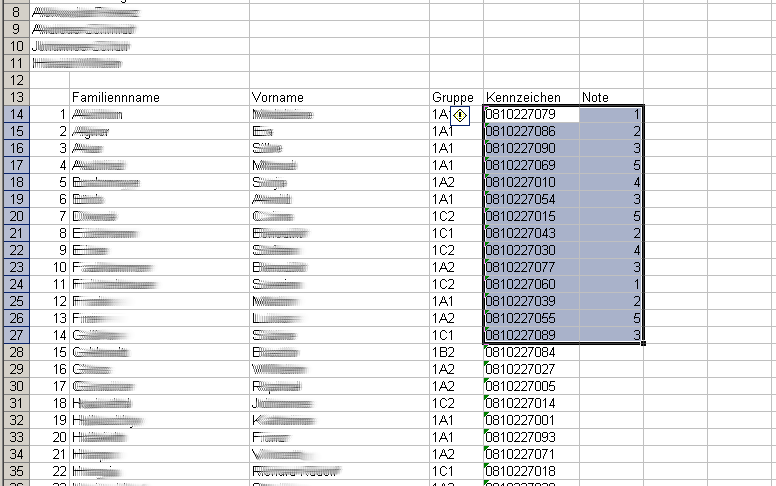
\includegraphics[width=1.0\textwidth]{CIS_Gesamtnote_Excelimport.png}
\end{center}
\caption{Excelimport}\label{excelimport}
\end{figure}
\item Kopieren Sie die markierten Spalten mittels $<$strg$>$+$<$c$>$ oder Bearbeiten-$>$Kopieren in die Zwischenablage
\item Mit einem Klick auf den Knopf 'Import' werden die Noten �bernommen.
\end{enumerate}
\achtung {Bestehende Noten werden ohne Nachfrage �berschrieben}
Damit der Notenimport funktioniert m�ssen im Browser einige Sicherheitseinstellungen vorgenommen werden:

\begin{enumerate}
\item Firefox / Mozilla
	\begin{enumerate}
	\item �ffnen Sie ein neues Browserfenster
	\item geben sie 'about:config' in die Adressleiste ein. 
	(M�glicherweise erscheint hier eine Warnmeldung die Sie mit einem klick auf den angezeigten Knopf �berspringen)
	\item Suchen sie den Eintrag 'signed.applets.codebase\_principal\_support'
	\item mit einem Doppelklick muss diese Einstellung auf 'true' gesetzt werden
	\end{enumerate}
	\achtung {Durch die Aktivierung dieses Eintrages wird ein Sicherheitsloch ge�ffnet. Wir empfehlen daher diese Einstellung nach dem
	Import wieder zur�ckzusetzen.}
\item InternetExplorer
	\begin{enumerate}
	\item Beim IE m�ssen keine Einstellungen vorgenommen werden. Wenn auf 'Import' geklickt wird erscheint (bei IE7) eine Warnungmeldung die sie mit 'Zugriff zulassen' best�tigen m�ssen.
	\end{enumerate}
\item Safari, Opera
	\begin{enumerate}
	\item Mit den Browsern Safari und Opera kann der Notenimport NICHT verwendet werden. Bitte verwenden Sie Firefox oder den InternetExplorer
	\end{enumerate}
\end{enumerate}

\subsection{Freigabe der Noten}
\label{freigabe}

Wenn Sie alle Noten eingetragen haben, die  Sie zu diesem Zeitpunkt
eintragen wollen (Sie k�nnen jederzeit Noten nachtragen!) k�nnen Sie diese
�ber den Knopf 'Freigabe' (im Tabellenkopf) f�r die AssistentIn freigeben.
(2)

\info {
ACHTUNG!! aus Gr�nden der erh�hten Sicherheit ist bei der Freigabe der Noten
die Eingabe Ihres Passwortes erforderlich.\footnote{Es handelt sich dabei um Ihr
TW-Passwort, mit dem sie sich auch auf der CIS-Seite authentifizieren oder auf
unseren Rechnern einloggen}
}

\begin{itemize}
	\item Zul�ssige Noten: 1-5, 7 (nicht beurteilt), 8 (teilgenommen)
	\item Bei der Freigabe wird ein Info-Email an Sie und die zust�ndige
	Studiengangs\-assistentIn geschickt. Enthalten sind Mat. Nr., Vorname,
	Nachname und Note der neuen oder ge�nderten Eintr�ge.
	\item Freigegebene Eintr�ge sind mit einem gr�nen Kreis mit H�kchen gekennzeichnet.
	\item Wenn Sie bereits freigegebene Noten ver�ndern, werden diese mit einem grauen Kreis mit H�kchen markiert (als Hinweis f�r Sie, dass die AssistentIn dar�ber noch nicht per Mail informiert wurde. Sie sieht allerdings diese neue Note sofort in ihrer Oberfl�che)
	\item Die freigegebenen Noten kann die AssistentIn nun als Zeugnisnote �bernehmen, die dann im n�chsten Feld f�r Sie zur Kontrolle angezeigt wird.
	\item Wenn sich die Zeugnisnote von der von Ihnen freigegebenen Note unterscheidet wird erstere rot umrandet markiert.
\end{itemize}

\subsection{Eintragen einer Nachpr�fung (2. Termin)}
\label{nachpruefung}

Sobald Sie eine LV-Note eingetragen und haben erscheint (bei Neuladen der
Seite, etwa durch die Freigabe der Noten) rechts neben der Zeugnisnote ein
Knopf zum Anlegen einer Nachpr�fung. Sobald eine solche angelegt ist sehen Sie
Datum und Note, sowie einen Editier-Knopf (s. Abb.
\ref{benotung_lv_nachpruefung_quick} (1),(2)).

\begin{figure}[ht]
\begin{center}
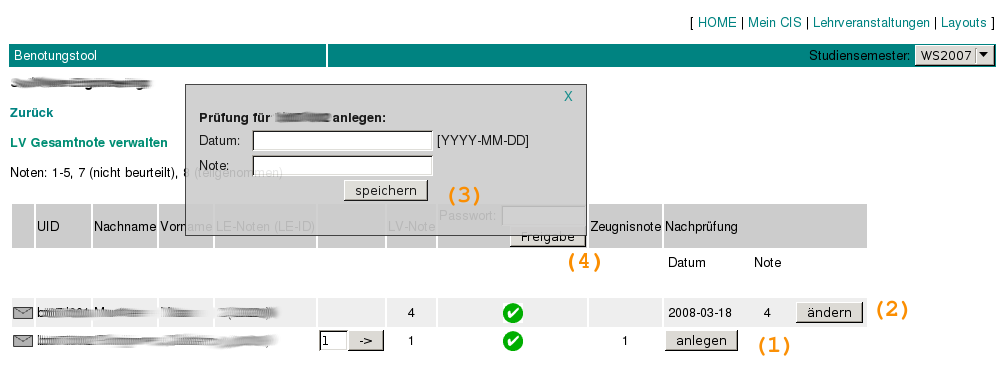
\includegraphics[width=1.0\textwidth]{benotungstool_benotung_lv_nachpruefung.png}
\end{center}
\caption{Benotung LV Nachpr�fung}\label{benotung_lv_nachpruefung_quick}
\end{figure}

Klicken Sie auf den jeweiligen Button, um eine Nachpr�fung anzulegen oder zu
editieren. Es �ffnet sich eine Eingabemaske (3) wo Sie Datum und Note eingeben und
mit Klick auf den 'speichern'-Knopf �bernehmen.

\begin{itemize}
    \item Beachten Sie bei der Einagbe bitte das Datumsformat: JJJJ-MM-DD
    \item Als Notenwerte sind wieder 1-5, 7 (nicht beurteilt), 8
    (teilgenommen) und hier zus�tzlich 9 (noch nicht eingetragen) zul�ssig. 
    Wenn Sie das Notenfeld leer lassen, wird dies als 9 interpretiert.
    \item Vergessen Sie nicht nach dem Eintragen neuer Noten diese erneut
    mithilfe des Buttons 'Freigabe' freizugeben (4).
\end{itemize}

%\newpage


